\documentclass{elsarticle}
\usepackage[latin1]{inputenc}
\usepackage[english]{babel}
%\usepackage[T1]{fontenc}
%\usepackage{textcomp}
\usepackage{graphicx}
\usepackage{color}
%\usepackage{setspace}
\usepackage{url}

\begin{document}

\begin{frontmatter}

%%%%%%%%%%%%%%%%%%%%%%%%%%%%%%%   TITLE   %%%%%%%%%%%%%%%%%%%%%%%%%%%%%%%

\title{Nowcasting traffic}


%%%%%%%%%%%%%%%%%%%%%%%%%%%%%%%   AUTHORS   %%%%%%%%%%%%%%%%%%%%%%%%%%%%%%%

\author{A.J. Fern�ndez-Ares$^1$, A.M. Mora$^1$, M.G. Arenas$^1$, P. Garc�a-Sanchez$^1$, G. Romero$^1$, V. Rivas$^2$, P.A. Castillo$^1$, J.J. Merelo$^1$}
\ead{\{antares, amorag, mgarenas, pablogarcia, gustavo, pacv, jmerelo\}@ugr.es, vrivas@ujaes.es}
\address{$^1$ Departamento de Arquitectura y Tecnolog�a de Computadores.\\ ETSIIT - CITIC. University of Granada, Spain\\
$^2$ Departamento de Inform�tica. EPS. Universidad de Ja�n, Spain}


\begin{abstract}
Traffic flow measurement methods must keep a balance between being
comprehensive but expensive and cumbersome, such as traffic spirals, also
called {\em loops}, or being cheap and mobile but missing some vehicles. 
In the framework of a smart city project, our group has been
developing MOBYWIT, a device that detects unique Bluetooth and Wifi
MACs and thus is able to measure their generated traffic, but also to uniquely identify
 bearers so that we can find out the actual path a particular
vehicle has followed. However, not all vehicles have a Bluetooth device installed yet,
and the ratio of vehicles with Bluetooth varies
along the day, the time of the day, and characteristics of the road. 
In this work our objective is to ``nowcast'', that is, to predict the actual number of vehicles, using
all available information, 
 including the number of vehicles bearing a wireless device. 
% I can not understand the previous sentence. Is it correctly written?   [pedro]
% I've rewritten it [Paloma]
We use classic and neural network techniques on data gathered in
installations where we have both kinds of devices, MOBYWIT and spirals,
%to try and find out some rules and give a more accurate estimate of the real number of cars in a particular road.
obtaining good accuracies in the estimation of the real number of cars in a particular road.
\end{abstract}

%
%%%%%%%%%%%%%%%%%%%%%%%%%%%%%%%%%   KEYWORDS   %%%%%%%%%%%%%%%%%%%%%%%%%%%%%%%%%
%
\begin{keyword}
Smart traffic \sep Transit indicators \sep Traffic forecast \sep Mobility analysis \sep Smart City \sep Internet of Things
\end{keyword}

\end{frontmatter}


%-------------------------------------------------------------------------------
%%%%%%%%%%%%%%%%%%%%%%%%%%%%%%%   INTRODUCTION   %%%%%%%%%%%%%%%%%%%%%%%%%%%%%%%
%-------------------------------------------------------------------------------

\section{Introduction}
\label{sec:intro}

Monitoring traffic and knowing the exact amount of vehicles that are
occupying a street in a particular moment is an issue where you have
to balance accuracy and price or convenience. Spirals, also called
traffic loops, 
\cite{klein2006traffic} embedded in the
road can give you the exact number of vehicles and even its type;
however, besides being expensive \textit{per se}, the road has to be opened
and re-asphalted to install them so they cannot be installed at short
notice. On the other hand, devices such as MOBYWIT
\cite{Castillo2014caplibro, DBLP:conf/smartct/Fernandez-AresA16}, which use some feature of
vehicles such as the emitting devices in them, only count part of the
devices and thus their accuracy is limited; incidentally, systems such
as the one used by Google Maps also rely on mobile devices
transmitting their location and thus do not cover the totality of
vehicles.

On the other hand, the accurate knowledge of the amount of traffic is
direly needed in the context of Smart Cities in order to avoid
congestions and also be able to plan routes in advance. In this
context, a solution can be using the less-accurate devices, which can
be deployed in a massive amount of places, to {\em now-cast}, that it,
predict, the actual traffic passing by a particular point in that
precise moment. 

In this paper, we will use data collected in the course of the PETRA \footnote{\url{https://proyectopetra.wordpress.com/}}
%FERGU: el problema es que la web de PETRA est� en espa�ol, pero la pongo por si acaso
% �se podr�a poner una secci�n en ingl�s (un abstract al menos) y quien vaya a visitarla, que pueda entrar.  [pedro]
project to find out, from available data, the actual vehicle count in
a place, obtained from the more precise spirals. We will use standard and bioinspired methods, and try to find
%FERGU: se va a usar tambi�n los datos de espiras para validar? Si es
%as�, indicarlo aqu��
%hecho - JJ
what could be the best option for the volume and type of data
available. Data, as well as its processing, is available in a GitHub
repository as part of the Open Science policy of our group. 
% �podemos poner la URL en nota a pie de p�gina?   [pedro]

The rest of the work is structured as follows. Section \ref{sec:soa}
presents the background and state of the art. Then, our monitoring device is introduced in Section
\ref{sec:mobywit}. The results on trying to use different prediction
methods are described in section 
Finally, Section \ref{sec:conclusions} plots the conclusions that we
have reached in the work. 


%----------------------------------------------------------------------------
%%%%%%%%%%%%%%%%%%%%%%%%%%%%%   STATE OF THE ART  %%%%%%%%%%%%%%%%%%%%%%%%%%%
%----------------------------------------------------------------------------


\section{Background and state of the art}
\label{sec:soa}

Nowcasting \cite{tepper1971weather} is just a way of predicting the value of data, and thus is
not really a new methodology; it refers to the type of data being
predicted, that is, the value of some variable at the same time as the
input variables, than to the actual way used to predict it. Initially,
it was applied to weather conditions, then was adopted by economics,
and eventually extended to any field. 
%FERGU: is nowcasting a new term invented by us? If not, add citation.
%Done - JJ
 However, as far as we have been able to find out, it has not been
 applied to vehicle traffic in the way we do in this paper. In
 \cite{hanabusa2013development} a model is used to nowcast traffic,
 instead of partial measurements, and in
 \cite{scharsching1996nowcasting} road conditions are predicted; in
 fact, many of the nowcasting applications are related to weather and
 merge data from different sources in order to predict with a certain
 spatial accuracy weather conditions. 

Our previous work has been mainly devoted to the design and
description of the monitoring device itself
\cite{Castillo2014caplibro,DBLP:conf/smartct/Fernandez-AresA16}. In this paper, after
% �podemos citar el cap�tulo de libro? Lo a�ado por si acaso  ;)  [pedro]
describing the system in the next section, we will use available data
to predict real traffic.  


%------------------------------------------------------------------------------
%%%%%%%%%%%%%%%%%%%%%%%%%%%%%%%%%%  MOBYWIT  %%%%%%%%%%%%%%%%%%%%%%%%%%%%%%%%%%
%------------------------------------------------------------------------------

\section{MOBYWIT}
\label{sec:mobywit}

The proposed device, which we call MOBYWIT (Mobility monitoring by Wireless Tracking)  is a single-board computer, based on the Raspberry
Pi\footnote{https://es.wikipedia.org/wiki/Raspberry\_Pi}. It includes
BT and WiFi devices connected via USB and configured in monitor mode
so that they can scan the radioelectric space searching for BT devices
and beacon frames (for WiFi).

In every device the monitoring system is formed by a closely coupled
hardware and software layer. The device has to be connected to the
Internet and stores data in the cloud. The software architecture of the system is shown in Figure \ref{fig:mobywit}. 

\begin{figure}[ht]
	\begin{center}
		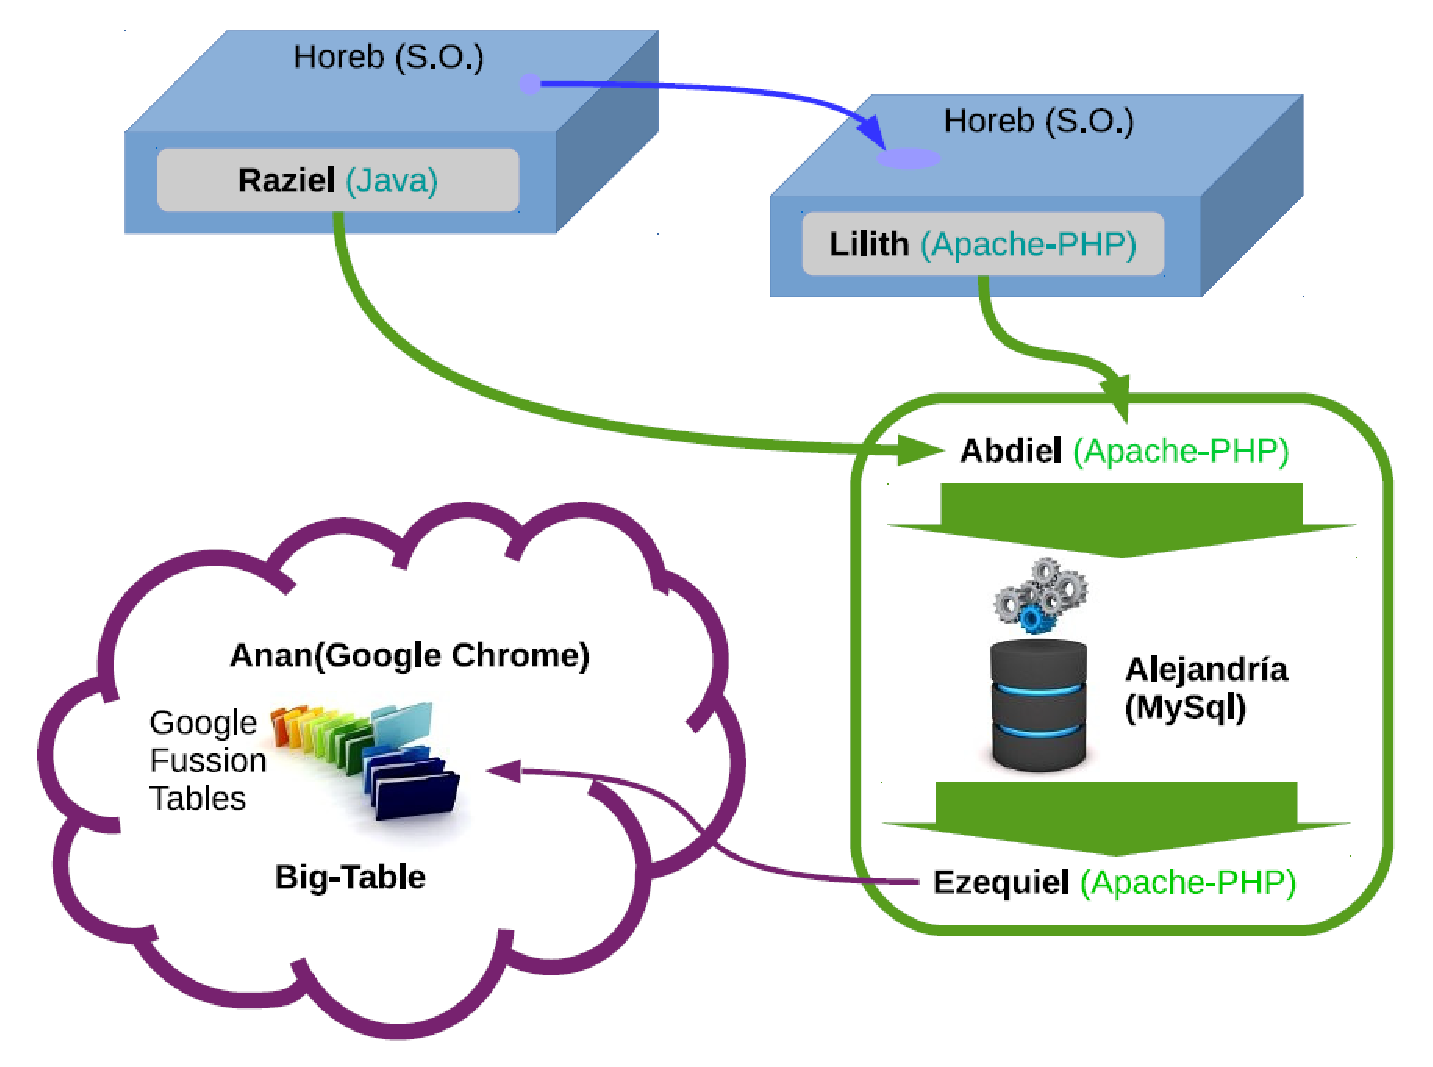
\includegraphics[scale=0.4]{imgs/mobywit.eps}
		\caption{MOBYWIT Monitoring system architecture}
	\label{fig:mobywit}
	\end{center}
\end{figure}

Figure \ref{fig:mobywit} shows the six main parts in the software
layer of the system, which are unidirectionally connected by a strict
data flow. These parts perform the following functions:
\begin{itemize}

\item \textit{Raziel} is in charge of the detection of BT and WiFi
  devices as well as of their identification, that is, extracting and
  encrypting the MAC,  as well as the periodic submission of this information
  to the server. It runs on the device and has been implemented in
  Java.

\item \textit{Lilith} acts as a gateway between the network of devices
  and the server, enabling the communications between nodes and between them and external networks. This component is also run on every device and implemented in PHP.

\item \textit{Abdiel}: This component implements a set of services for accessing the devices from `outside' (mainly for activate/deactivate or update them). In addition, it performs the storage of gathered data (in blocks) in the server database. It is also implemented in PHP.

\item \textit{Alejandr�a} is the database managing subsystem, a MySQL
  instance placed in a local server. It is optimised using b-tree
  indexes, stored procedures, table partitioning and temporally memory
  tables to provide a close to real-time processing and data service. 

\item \textit{Ezequiel} is responsible for the publication of data in
  a cloud-based storage. It includes data mining, machine learning and
  forecasting techniques that act on the data in order to publish
  interesting or useful information about them. 

\item \textit{Anan} is the cloud-based storage and services. It is
  based on Google technology, storing the data in a NoSQL format by
  means of Google Fusion Tables. It also offers advanced visualisation
  methods to be more usable and attractive to the end-user of the
  system. 

\end{itemize}

%FERGU: if there is space constriction we could remove the parts of the system (already explained in other papers)
In addition the device runs a customized Operating System, called
\textit{Horeb}, a modification of the original Raspbian 3.10.24,
adapted by us to be more robust (to power failures, for instance) and
reliable.

There are several configuration parameters in the system, which set
important parts of the functionality, such as the intensity threshold
to collect a received WiFi signal, or time limits to consider a device
as obsolete or out of the range of the device. 

Every detected `pass-by' or mobility `event' is associated with a
detection time, obtained by NTP (Network Time Protocol). These
`events' are stored initially in the device's memory, but after some
time (also set in a parameter) the information is sent, in blocks, to
the server, to avoid an overuse/saturation of the network and also
save bandwidth.

From the point of view of this paper, MOBYWIT will collect the number
of devices detected in a particular period of time; so the data we
will have will be a timestamp and a vehicle count. 

\section{Nowcasting traffic}
\label{sec:nowcasting}

Our intention in this paper, and particularly in this section, is to
show that, in fact, there is a high correlation between the number of
vehicles detected and the actual number of vehicles. 
% este objetivo creo que deber�a aparecer en el abstract. 
% Es una buena frase para resumir el objetivo principal del paper  [pedro]
In order to check
it, the Spanish national traffic directorate (DGT) made available data from their
own spirals, situated near or in the same place as our MOBYWIT. This
data is available from the same repository as this paper,
\url{https://github.com/geneura-papers/nowcasting-traffic}. These data
are from a single month in a single year, and only during 3 hours,
although we have different days the week. The data is not too
comprehensive, but at least gives us an idea of how the existing
factors might influence the outcome. 


One of the things we will have to take into account is that our device
only detects WiFi and Bluetooth devices. In the case of vehicles, it
is mainly hands-free Bluetooth devices. These devices have to be
installed and connected to be detected, unlike WiFi devices that do
not actually need to be activated; however, very few vehicles nowadays
actually include these devices. Only a fraction of vehicles will be
equipped with any of them, and this amount will change with the time
of the day and also the type of road; while you might expect many more
hands-free devices in urban areas, there might not be as many in rural
areas. Probably the time of the day and the type of traffic,
commuters, services or professional traffic will also present a very
different profile. While commuters might have a lower amount of BT
devices, services or professional will almost always have one. That is
why even as we know that it will always be a fraction, the actual
number will change depending on many different factors. 

In the next subsection we will use only the number of detected
vehicles for nowcasting. In Subsection \ref{ss:nc} we will test
different methods and also different variables to increase the
accuracy.

\subsection{Correlation between detected and actual number of vehicles}

Different metrics will be used to obtain a correct correlation between
the number of detected devices and the real number detected by the
loop detectors.  In this subsection we will only look at these two
variables to check the relationship between them. We will examine the
following ratios:

\begin{itemize}
\item {\em Total ratio}: ratio between the total number of vehicles
  detected by the DGT and the total number of vehicles detected by our
  device. 
\item {\em Mean ratio}: as the maximum granularity of the data
  provided by the DGT is 15 minutes, the sum of all ratios between the
  DGT data and our data in each 15 minute section has been divided by
  the total number of sections to calculate the average. 
\item {\em Median ratio}: instead the average ratio as in previous
  metric, this one uses the median of all ratios. 
\item {\em Mean by quarter ratio}: this metric calculates a vector of
  ratios separated by quarter of hour during the day, instead
  obtaining a global ratio for all data. An average ratio per quarter
  per hour in the vector is calculated taking into account all the
  ratios of that quarter during all the days we have data. 
\item {\em Median by quarter ratio}: as in the previous metric, this one uses a vector of ratios per quarter of hour, but every element is calculated using the median, instead the average.
\end{itemize}

Table \ref{tab:ratiosDGT} shows the obtained ratios. To simplify the
data analysis and discussion only the data for one node ({\tt 1010}) is
shown. In general, our device detects one vehicle per
approximately 19 detected by the DGT, according to Total, Mean and Median
ratios. However, best results in MAE and MAPE are attained obtaining
ratios dividing by quarter. 

\begin{table}[htb]
\centering
\resizebox{12cm}{!}{
\begin{tabular}{|l|l|l|l|l|l|}
\hline
			 &RATIO	  & MAE    &   MAPE   & MSE    & RMSE \\
 \hline
Total Ratio  & 17.230 &   60.373 & 36.265 & \textbf{7371.579}  & \textbf{85.857} \\
Mean Ratio   & 20.792 &   72.323 & 43.443 & 11216.070 & 105.905 \\
Median Ratio & 18.2 &    62.454  & 37.515 & 8060.136  & 89.778 \\
Mean By Quarter of Hour Ratio &   Depends on the hour  & 66.791 & 40.120 & 9890.978 & 99.453 \\
Median By Quarter of Hour Ratio & Depends on the hour  & \textbf{58.326} & \textbf{35.035} & 7617.613 & 87.278 \\
\hline

\end{tabular}
}
\caption{Different ratios between the DGT data and the data gathered by MOBYWIT in node 1010.}
\label{tab:ratiosDGT}
\end{table}

Figure \ref{fig:dgtRatios} shows the number of devices detected in node
{\tt 1010}, applying the chosen correction ratio. As it can be seen, certain
correlation exists. However, different peaks appear in the figure,
being those elements the product of detecting few devices in
comparison with the DGT. 

\begin{figure}[htb]
	\begin{center}
		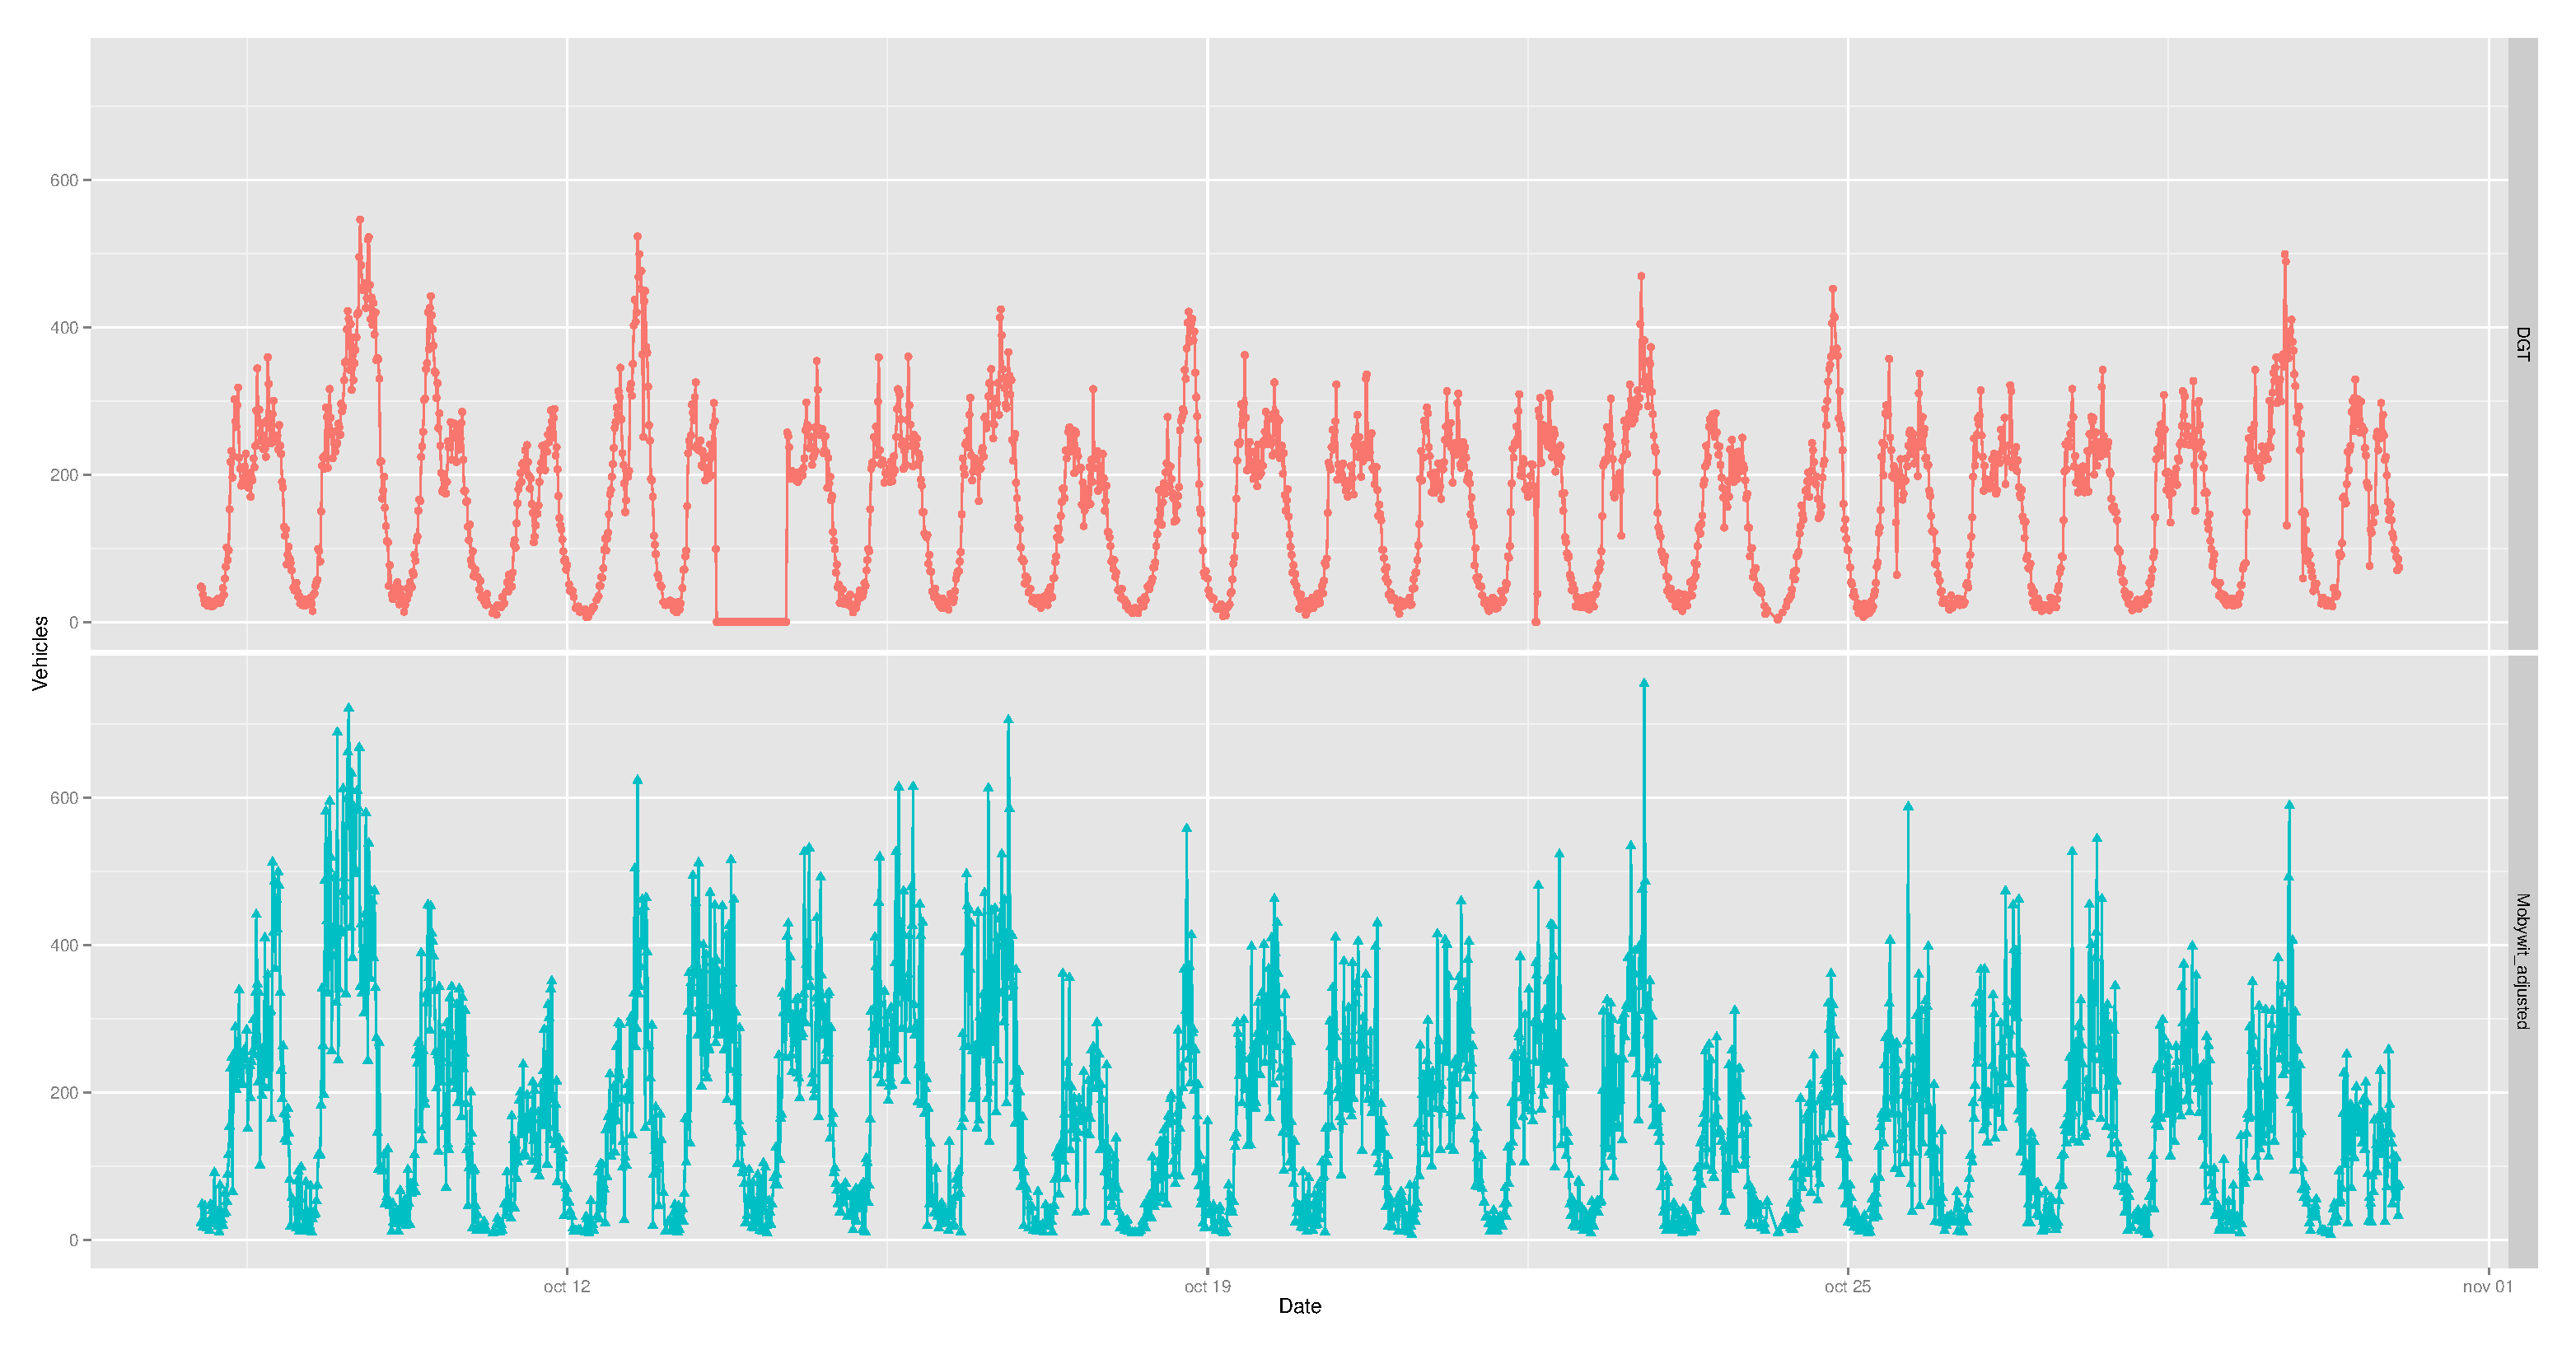
\includegraphics[scale=0.22]{imgs/petra_graph_DGT-Mobywit-mended.eps}
		\caption{Devices detected by DGT and detected by our device (node 1010) applying the correction ratio (median by quarter). Note: no DGT data available during October 14th.}
	\label{fig:dgtRatios}
	\end{center}
\end{figure}

The fact that the ratio of detected-to-actual vehicles is one in ten
makes nowcasting a challenge. In the next section we will show how we
can improve this result by using the context.

\subsection{Context-sensitive nowcasting}
\label{ss:nc}

The information provided by the loops and MOBYWIT includes little more
than the time. However, it is clear that the moment of the day and the
week has a clear influence on traffic, and it might also have an
influence on the ratio of vehicles detected. That is why in this
section we intend to train models taking into account the time: day of
the week and time of the day. The month would have also been used, but
all data available was for a single month, October, so it was not
eventually relevant.

We used the R datamining tool Rattle \cite{williams2009rattle} to
perform this task. Rattle allows to analyze data in different ways, as
well as train models and compare them with each other. We have tested
four different models: Regression Trees, Random Forest, Neural Networks
and a simple linear model. As an initial exploration, we
applied it to the data of a single node, {\tt 1011}. The results of
different methods, with R-square values, are shown in Figure
\ref{fig:1011fit}. 
%
\begin{figure}[htb]
	\begin{center}
		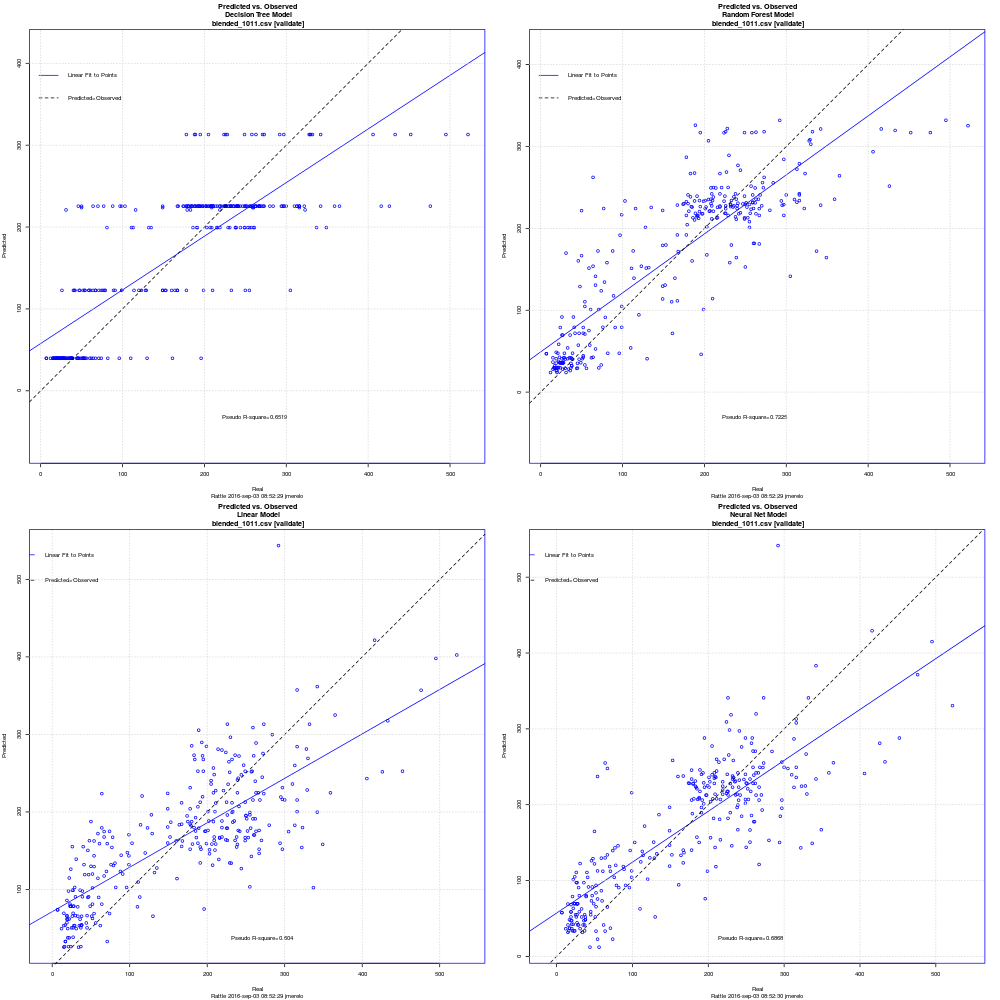
\includegraphics[scale=0.35]{imgs/blended_1011_plot.png}
		\caption{Different regression models applied to the
                  nowcasting of real traffic in node 1010. The graphs
                  include R-square values, with higher is better. All
                  graphs plot Real in the $x$ axis vs. predicted in
                  the $y$ axis.}
	\label{fig:1011fit}
	\end{center}
\end{figure}

As is usually the case, the Random Forest, with 200 trees, model shows the best
results, with an R-value of 0.7225. The backpropagation neural net
model, with 10 hidden nodes, does have a good regression value of
0.6868. The other two models show rather disappointing results, so
they will be discarded. 

It is interesting to note that the Random Forest, using the
conditional algorithm, actually uses the context. While assigning an
importance value of 7863.706 to the number of vehicles detected by
MOBYWIT, it also assigns 3932.992 to the hour and 1000.817 to the day
of the week. This indicates that these two context variables can
actually {\em improve} the value of the prediction that we have shown
before for just the detected value.

In order to confirme these findings using the whole dataset, we will
consider data from all detectors and blend them into a single file
with 4755 observations, all of them in the same month. Even if the
ratio of detected to actual might be different for different
detectors, we will try to find out what would be the accuracy of a
model that could be used in general for all detectors. Once again, we
will use Rattle, but limited to the two models with the best R-value,
Random Forest and Neural Net.
%
\begin{figure}[htb]
	\begin{center}
		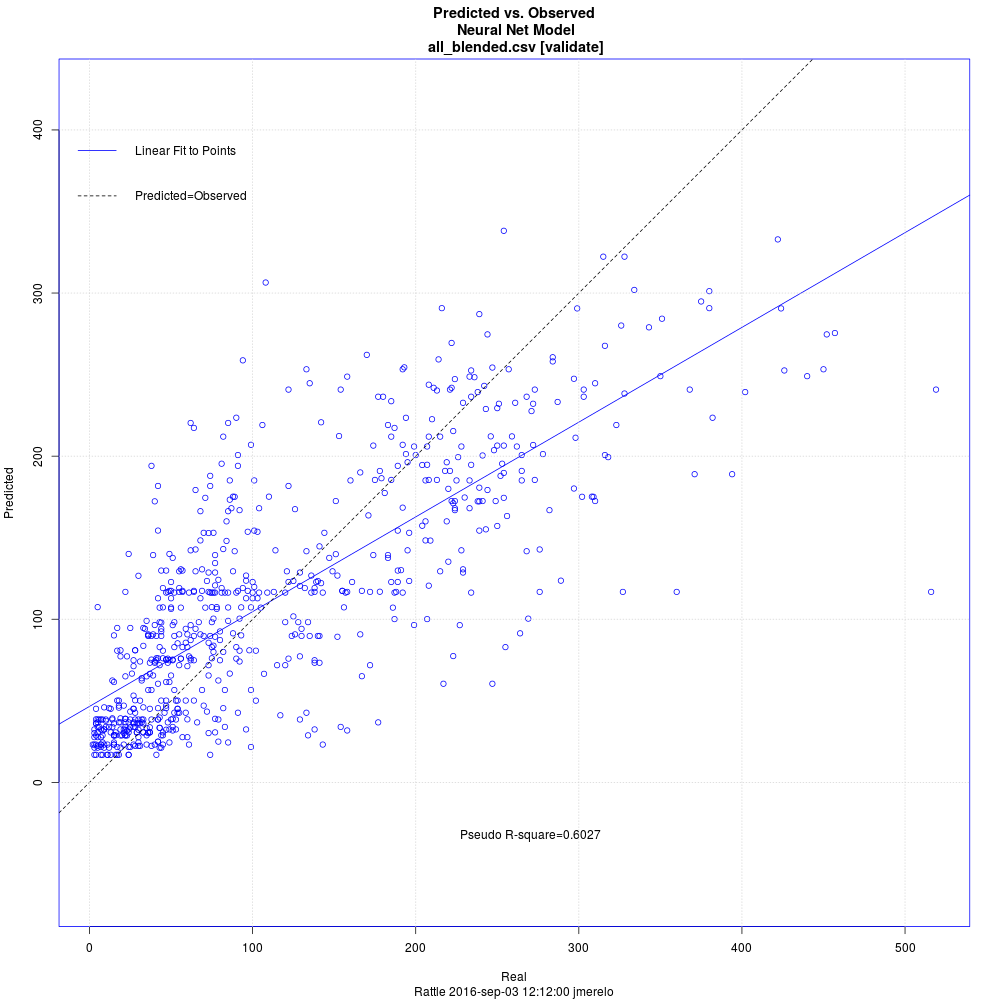
\includegraphics[scale=0.3]{imgs/all_blended_plot-nn.png}
		\caption{Result of fit of the whole data set via a
                  backpropagation neural net.}
	\end{center}
	\label{fig:allfit:nn}
\end{figure}
%
\begin{figure}[htb]
	\begin{center}
		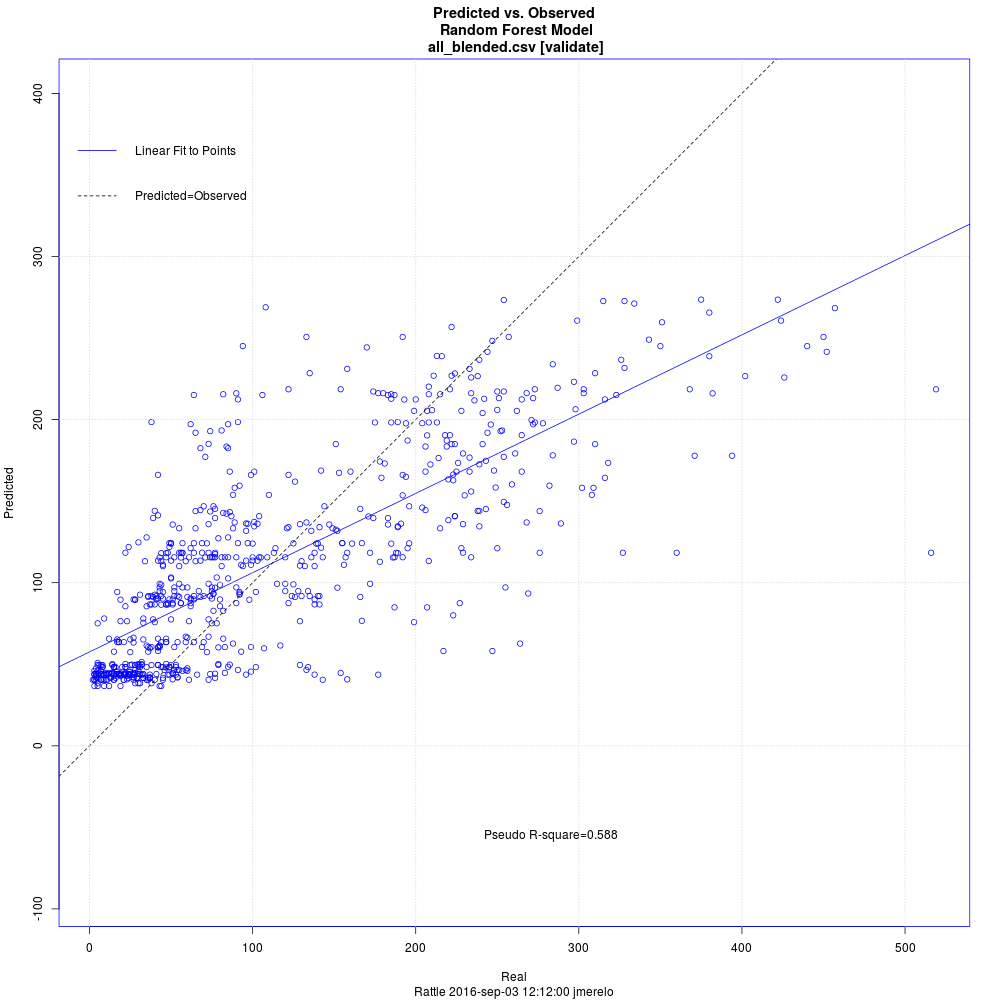
\includegraphics[scale=0.3]{imgs/all_blended_plot-rf.png}
		\caption{Result of fit of the whole data set via a random forest
                  (bottom). R-square value is inset.}
	\end{center}
	\label{fig:allfit:rf}
\end{figure}
%
Plot of observed-vs-actual for the backpropagation neural net is shown
in \ref{fig:allfit:nn} and for the random forest in
\ref{fig:allfit:nn}. In this case, R-square results are worse than
before, probably indicating that there is some specifity in the
particular sensors that have an influence in result. The neural net
obtains results that are slightly better with an R-square of around
0.60 for 20 hidden nodes; the random forest R-square falls to 0.59
with 400 trees. Besides, in this last case the hour matches its
importance to the detected values, indicating that the context, in
this case, is as important as the actual number of detected values;
the importance for the day of the week is 2/3rds of them, so, in fact,
context, that is, the day and the time of day have a high importance
when nowcasting the actual number of vehicles in the road at a
particular point in time. 

%----------------------------------------------------------------------------
%%%%%%%%%%%%%%%%%%%%%%%%%%%%%%%   CONCLUSIONS  %%%%%%%%%%%%%%%%%%%%%%%%%%%%%%%
%----------------------------------------------------------------------------

\section{Conclusions}
\label{sec:conclusions}

In general, as we set to prove in this paper, detecting a fraction of
vehicles using low-cost and mobile detectors such as MOBYWIT can help
determine the actual number of vehicles with an accuracy that is
around 70\% if sensor-specific data is available, or 60\% if it is
not. In general, models underestimate the actual number of vehicles,
and a backpropagation neural network trained with detected number of
vehicles as well as the day of the week and hour has proved to obtain
reliably good results, although it can be overcome by random forest if
sensor-specific data is available.

External factors not included in the model have a definite  influence
in the result, as exemplified that sensor-independent models have less
accuracy than sensor-specific ones. These might be type of road and
type of traffic, but a deeper study of road conditions and traffic
should be added to it. 

The amount of vehicles detected is also related to the actual location
of the sensor. Improving the antenna situation will definitely improve
the signals detected by MOBYWIT. 10\%, as shown by the initial study,
is really a low value and does not actually reflect the amount of
vehicles bearing BT or WiFi antennas, so this study is actually
telling us that a careful installation of antennas must be performed
to improve the accuracy of the prediction. %FERGU: we have not discussed about antenna location in the paper

These conclusions above also inform future lines of work, along the
lines of increasing context description and also the number of
vehicles detected. This will be done in the near future.

%%%%%%%%%%%%%%%%%%%%%%%%%%%%%  ACKNOWLEDGEMENTS %%%%%%%%%%%%%%%%%%%%%%%%%%%%%%%%

\section*{Acknowledgements}

This work has been supported in part by projects EPHEMECH
(TIN2014-56494-C4-3-P, Spanish Ministry of Economy and Competitivity),
PETRA (SPIP2014-01437, funded by Direcci�n General de Tr�fico),
PYR-2014-17 (GENIL project, awarded by CEI-BIOTIC Granada), 
PROY-PP2015-06 (Plan Propio 2015, funded by the University of Granada, Spain),
and MOSOS (PRY142/14, granted by Fundaci�n P�blica Andaluza Centro de
Estudios Andaluces in the call 'IX Convocatoria de Proyectos de Investigaci�n). 
We also thank the DGT and their staff and researchers for their dedication and
professionalism.  


% ---------------------- BIBLIOGRAF�A -----------------------

\bibliographystyle{elsarticle-num}
\bibliography{mobility,geneura-latin1}


\end{document}
